\section{Solving Identification with a Control Function (CF)}
\label{sec:selectionmodel}
If your goal is to estimate CM effects, and you could control for unobserved selection terms $U_{0,i}, U_{1,i}$, then you would.
This ideal (but infeasible) scenario would yield unbiased estimates for the ADE and AIE.
% Alas, $U_i$ is by definition unobserved.
A Control Function (CF) approach takes this insight seriously, providing conditions to model the implied confounding by $U_{0,i}, U_{1,i}$, and then controlling for it.

The main problem is that second-stage regression equation \eqref{eqn:parametric-secondstage} is not identified, because $U_{0,i},U_{1,i}$ are unobserved, and lead to omitted variables bias.
\begin{align}
    \Egiven{Y_i}{Z_i, D_i, \vec X_i} \;\; =& \;\;
        \alpha
        + \beta D_i
        + \gamma Z_i
        + \delta Z_i D_i
        + \varphi(\vec X_i) \nonumber \\
        \label{eqn:secondstage-reg}
        & \;\; +\underbrace{\left( 1 - D_i
            \right) \Egiven{ U_{0,i} }{D_i = 0, \vec X_i}
                + D_i \Egiven{ U_{1,i} }{D_i = 1, \vec X_i}}_{
                    \text{Unobserved confounding.}}
\end{align}

The CF approach models the contaminating terms in \eqref{eqn:secondstage-reg}, avoiding the bias from omitting them in regression estimates.
CF methods were first devised to correct for sample selection problems \citep{heckman1974shadow}, and were extended to a general selection problem of the same form as \autoref{eqn:secondstage-reg} \citep{heckman1979sample}.
The approach works in the following manner: (1) assume that the variable of interest follows a selection model, where unexplained first-stage selection informs unobserved second-stage confounding; (2) extract information about unobserved confounding from the first-stage; and (3) incorporate this information as control terms in the second-stage equation to adjust for selection-into-mediator.
Identification in CF methods typically relies on either distributional assumptions on the unobserved error terms, or an exclusion restriction for instrumental variables in the first-stage (or both).
By explicitly accounting for the information contained in the first-stage selection model, CF methods enable consistent estimation of causal effects in the second-stage even when selection is driven by unobserved factors \citep{florens2008identification}.

In the example of analysing health gains from health insurance \citep{finkelstein2008oregon}, a CF approach addresses the unobserved confounding from underlying health conditions.
It does so by assuming that unobserved selection-into-frequent health care usage is informative for underlying health conditions, assuming people with more severe underlying conditions visit the doctor more often than those without.
Then it uses this information in the second-stage estimation of how much the effect goes through increased healthcare usage, estimating the ADE and AIE.

\subsection{Re-identification of Causal Mediation (CM) Effects}
The following assumptions are sufficient to model the correlated error terms, identifying $\beta, \gamma, \delta$ in the second-stage regression \eqref{eqn:parametric-secondstage}, and thus both the ADE and AIE.

\theoremstyle{definition}
\newtheorem{assumptionCF}{Assumption}
\renewcommand\theassumptionCF{CF--\arabic{assumptionCF}}
\begin{assumptionCF}
    \label{cf:monotonicity}
    Mediator monotonicity, conditional on $\vec X_i$.
    \[ \Probgiven{ D_i(0) \leq D_i(1) }{\vec X_i} = 1. \]
\end{assumptionCF}
\noindent
Assumption \ref{cf:monotonicity} is the monotonicity condition first used in an instrumental variables context \citep{imbens1994identification}.
Here, it is assuming that people respond to treatment, $Z_i$, by consistently taking or refusing the mediator $D_i$ (always or never-mediators), or taking the mediator $D_i$ if and only if assigned to the treatment $Z_i=1$ (mediator compliers).
There are no mediator defiers.

The main implication of Assumption \ref{cf:monotonicity} is that selection-into-mediator can be written as a selection model with ordered threshold crossing values that describe selection-into-$D_i$ \citep{vytlacil2002independence}.
\[ D_i(z') = \indicator{V_i \leq \psi \big( z'; \vec X_i \big)},
    \;\text{ for } z'=0,1 \]
where $V_i$ is a latent variable with continuous distribution and conditional cumulative density function $F_V(. \,|\vec X_i)$, and $\psi(. \,;\vec X_i)$ collects observed sources of mediator selection.
$V_i$ could be assumed to follow a known distribution; the canonical Heckman selection model assumes $V_i$ is normally distributed (a ``Heckit'' model).
The identification strategy here applies to the general case that the distribution of $V_i$ is unknown, without parametric restrictions.

I focus on the equivalent transformed model of \cite{heckman2005structural},
\[ D_i(z') = \indicator{U_i \leq \pi(z'; \vec X_i)},
    \;\;\; \text{for } z'=0,1 \]
where $U_i \coloneqq F_V\left( V_i \mid \vec X_i \right)$ follows a uniform distribution, and $\pi(z'; \vec X_i) = F_V\big(\psi(z'; \vec X_i)\big) = \Probgiven{D_i = 1}{Z_i = z', \vec X_i}$ is the mediator propensity score.
$U_i$ are the unobserved mediator take-up costs.
Note the maintained assumption that treatment $Z_i$ is ignorable conditional on $\vec X_i$ implies $Z_i \indep U_i$ conditional on $\vec X_i$.

This selection model setup is equivalent to the monotonicity condition, and is importing a well-known equivalence result from the instrumental variables literature to the CM setting.
The main conceptual difference is not assuming $Z_i$ is a valid instrument for identifying $D \to Y$ effects among compliers; it is using the selection model representation to correct for selection bias.
See \aref{appendix:cf-monotonicity} for a validation of the general \cite{vytlacil2002independence} equivalence result in a CM setting, with conditioning covariates $\vec X_i$.

\begin{assumptionCF}
    \label{cf:identification}
    Selection on mediator costs and benefits.
    \[ \Cov{U_i, \, U_{0,i}}, \; \Cov{U_i, \, U_{1,i}} \neq 0. \]
\end{assumptionCF}
\noindent
Assumption \ref{cf:identification} is stating that unobserved selection in mediator take-up ($U_i$) informs second-stage confounding, when refusing or taking the mediator ($U_{0,i}$ and $U_{1,i}$).

This is a strong assumption, and will not hold in all examples.
If people had been deciding to take $D_i$ by a Roy model, then this assumption holds because $V_i = U_{C,i} - \big( U_{1,i} - U_{0,i} \big)$.
Individuals could be making decisions based on other outcomes, but as long as mediator costs and benefits guide at least part of this decision (i.e., bounded away from zero), then this assumption will hold.

For notation purposes, suppose the vector of control variables $\vec X_i$ has at least two entries;
denote $\vec X_i^{\text{IV}}$ as one entry in the vector, and $\vec X_i^-$ as the remaining.
\begin{assumptionCF}
    \label{cf:instrument}
    Mediator take-up cost instrument.
    \[ \vec X_i^{\text{IV}} \textnormal{ satisfies } \;
    \partialdiff{\vec X_i^{\text{IV}}}\Big\{
        \mu_1(z', \vec X_i) - \mu_0(z', \vec X_i) \Big\} = 0
        < \partialdiff{\vec X_i^{\text{IV}}}
        \Big\{
            \Egiven{D_i(z')}{\vec X_i}\Big\},
        \textnormal{ for } z' = 0, 1. \]
\end{assumptionCF}
\noindent
Assumption \ref{cf:instrument} is requiring at least one control variable guides selection-into-$D_i$ --- an Instrumental Variable (IV).
It assumes an instrument exists, which satisfies an exclusion restriction (i.e., not impacting mediator gains $\mu_1-\mu_0$), and has a non-zero influence on the mediator (i.e., strong IV first-stage).
The exclusion restriction is untestable, and must be guided by domain-specific knowledge; IV first-stage strength is testable, and must be justified with data by methods common in the IV literature.

This assumption identifies the mediator propensity score separately from the direct and indirect effects, avoiding indeterminacy in the second-stage outcome equation.
While not technically required for identification, it avoids relying entirely on an assumed distribution for unobserved error terms (and bias from inevitably breaking this assumption).
The most compelling example of a mediator IV is using data on the cost of mediator take-up as a first-stage IV, if it varies between individuals for unrelated reasons and is strong in explaining mediator take-up.

\begin{proposition}
    \label{proposition:secondstage}
    If assumptions \ref{cf:monotonicity}, \ref{cf:identification}, \ref{cf:instrument} hold, then second-stage regression equation \eqref{eqn:parametric-secondstage} is identified with a CF adjustment.
    \begin{align*}
        \Egiven{Y_i}{Z_i, D_i, \vec X_i} \;\; =& \;\;
            \alpha
            + \beta D_i
            + \gamma Z_i
            + \delta Z_i D_i
            + \varphi\big(\vec X_i^-\big) \\
            & \;\; +  \rho_0 \left( 1 - D_i \right) \lambda_0 \big( \pi(Z_i ; \vec X_i) \big)
                + \rho_1 D_i \lambda_1 \big( \pi(Z_i ; \vec X_i) \big),
            \label{eqn:cf-secondstage}
    \end{align*}
    where $\lambda_0, \lambda_1$ are the Control Functions (CFs), $\rho_0, \rho_1$ are linear parameters, and mediator propensity score $\pi(z';\vec X_i)$ is separately identified in the first-stage \eqref{eqn:parametric-firststage}.
    Proof: see \aref{appendix:cf-secondstage}.
\end{proposition}
Again, this set-up required no linearity assumptions, treatment effects vary because$Z_i, D_i$ are categorical and  $\beta, \gamma, \delta , \varphi(\vec X_i)$ vary with $\vec X_i$.
The CFs are functions which measure unobserved mediator gains, for those with unobserved mediator costs above or below a propensity score value.
Following the IV notation of \cite{kline2019heckits}, put $\mu_V = \E{F_V^{-1}\left( U_i \mid \vec{X}_i \right)}$, to give the following representation for the CFs:
\begin{align*}
    \lambda_0\big(p'\big) &=
        \Egiven{ F_V^{-1}\left( U_i \mid \vec{X}_i \right) - \mu_V}{p' < U_i}, \\
    \lambda_1\big(p'\big) &=
        \Egiven{ F_V^{-1}\left( U_i \mid \vec{X}_i \right) - \mu_V}{U_i \leq p'} = 
            -\lambda_0\big( p' \big) \left(\frac{1-p'}{p'}\right), \text{ for } p' \in (0,1).
\end{align*}

If we are using the canonical Heckman selection model, we assume the error term follows a normal distribution, so that $\lambda_0, \lambda_1$ are the inverse Mills ratio.
Alternatively, $\lambda_0, \lambda_1$ could have other definitions following the assumed distribution of the error terms (see e.g, \citealt{wooldridge2015control}).
If we do not know what distribution class the errors follow, then $\lambda_0, \lambda_1$ can be estimated separately with semi-parametric methods to avoid relying on parametric assumptions.
%(as in \autoref{sec:semi-parametric}.

\newtheorem{theoremCF}{Theorem}
\renewcommand\thetheoremCF{CF}
\begin{theoremCF}
    \label{thm:cf-identification}
    If assumptions \ref{cf:monotonicity}, \ref{cf:identification}, \ref{cf:instrument} hold, the ADE and AIE are identified as a function of the parameters in Proposition \ref{proposition:secondstage}.
    \begin{align*}
    \text{ADE}
    %= \E{Y_i(1, D_i(Z_i)) - Y_i(0, D_i(Z_i))}
        &= \E{\gamma + \delta D_i}, \\
    \text{AIE}
    %= \E{Y_i(Z_i, D_i(1)) - Y_i(Z_i, D_i(0))}
        &= \mathbb E \Bigg[ \, \bar \pi \,
            \Big( \beta +  \delta Z_i +
                \underbrace{ (\rho_1 - \rho_0) \,
                \Gamma \big(\pi(0; \vec X_i), \, \pi(1; \vec X_i) \big)}_{
                    \text{Mediator compliers adjustment}} \Big) \Bigg]
    \end{align*}
    where $\Gamma\left(p,p'\right) 
    = \Egiven{ F_V^{-1}\left( U_i \mid \vec{X}_i \right) - \mu_V}{p < U_i \leq p'}
    = \frac{p'\lambda_1\left(p'\right) - p\lambda_1\left(p\right)}{p' - p}$ is the average unobserved net gains for those with unobserved costs between $p < p'$,\footnote{
        The complier adjustment term was first written in this manner by \cite{kline2019heckits} for an IV setting.
    } and $\bar\pi = \pi(1; \vec X_i) - \pi(0; \vec X_i)$ is the mediator complier score.
    Proof: see \aref{appendix:cf-ade-aie}.
\end{theoremCF}

This theorem provides a solution to the identification problem for CM effects when facing selection;
rather than assuming away selection problems, it explicitly models them.
The ADE is straightforward to calculate as an average of the direct effect parameters, while the AIE also includes an adjustment for unobserved complier gains to the mediator.
Again, this is because the AIE only refers to individuals who were induced by treatment $Z$ into taking mediator $D$ (mediator compliers).
The CFs allow us to measure both selection bias and complier differences, and thus purge persistent bias in identifying CM effects.

\begin{figure}[h!]
    \caption{The CF Adjustment Addresses Persistent Bias in CM Estimates.}
    \begin{subfigure}[c]{0.475\textwidth}
        \centering
        \caption{$\hat{\text{ADE}} - \text{ADE}$.}
        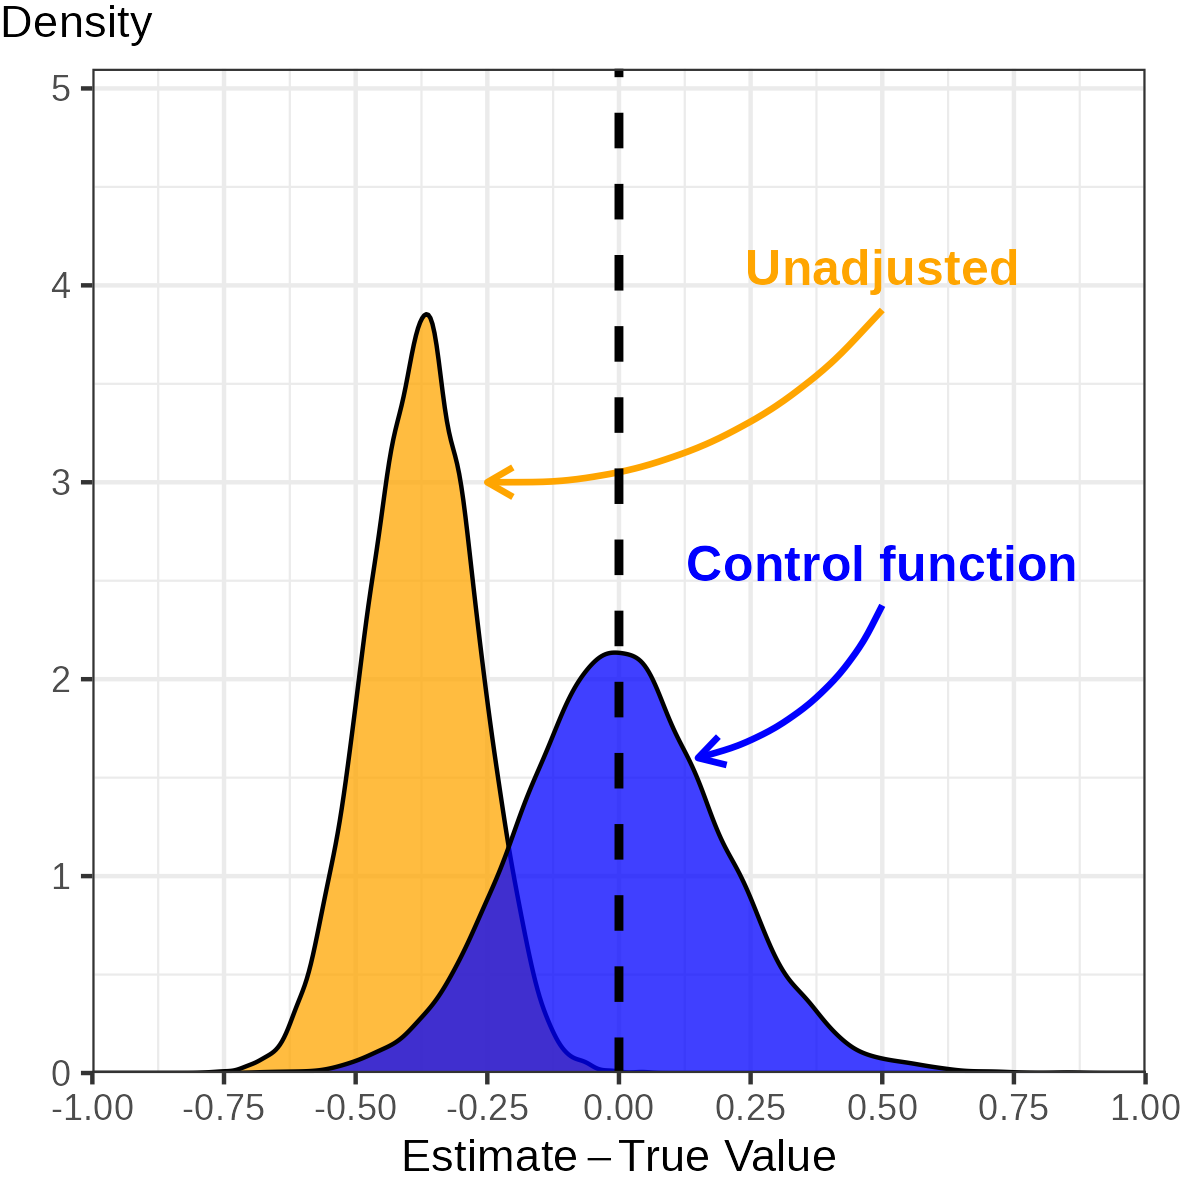
\includegraphics[width=\textwidth]{
            ../programs/simulations/sim-output/heckit-direct-dist.png}
    \end{subfigure}
    \begin{subfigure}[c]{0.475\textwidth}
        \centering
        \caption{$\hat{\text{AIE}} - \text{AIE}$.}
        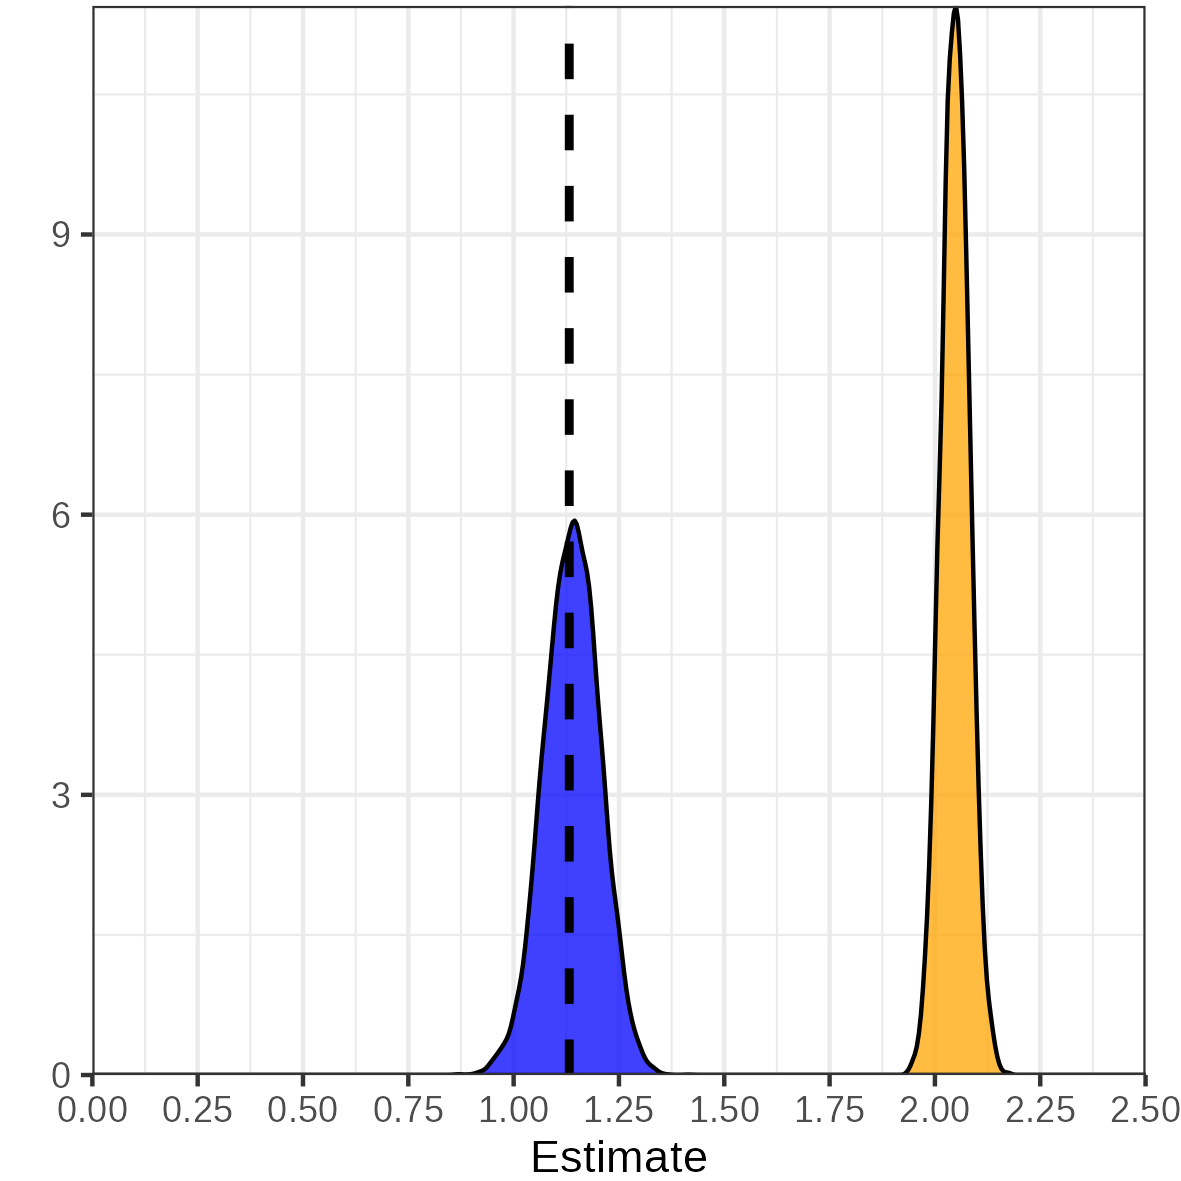
\includegraphics[width=\textwidth]{
            ../programs/simulations/sim-output/heckit-indirect-dist.png}
    \end{subfigure}
    \label{fig:cm-heckit-dist}
    \justify
    \footnotesize    
    \textbf{Note:}
    These figures show the empirical density of point estimates minus the true average effect, for 10,000 different datasets generated from a Roy model with correlated normally distributed error terms (further described in \autoref{sec:simulations}).
    The black dashed line is the true value;
    orange is the distribution of conventional CM estimates from two-stage OLS \citep{imai2010identification},
    and blue estimates with a two-stage Heckman selection adjustment.
\end{figure}

\autoref{fig:cm-heckit-dist} shows how a CF adjustment corrects unadjusted CM effect estimates.
In a simulation with selection-into-mediator based on unobserved error terms, the CF adjustment pushes conventional CM estimates back to the true value. 

% \subsubsection{Connection to Marginal Treatment Effects}
% It is worth noting that this approach is essentially an MTE approach (Marginal Treatment Effect, developed by Heckman and Vytlacil, 1999, 2005) applied to a causal mediation setting. Just as the semi-parametric local IV approach uses variation in instruments to identify marginal treatment effects across different resistance-to-treatment margins, our semi-parametric CF approach identifies mediation effects across the distribution of unobserved mediator gains. This connection to the MTE literature provides a conceptual bridge between the instrumental variables literature and causal mediation analysis.
